\documentclass{article}[12pt]
\usepackage{graphicx}

\title{[BSS]-Lab1-śr16-KrzysztofRudnicki}
\author{Krzysztof Rudnicki}
\begin{document} 
\maketitle 
\section{Generacja kluczy}
\paragraph{Wybrane liczby}
Wybrałem najniższe liczby pierwsze z przedziału 30 - 100 \\ 
p - 31, q - 37
\paragraph{Sprawdziłem że liczby 31 i 37 \textbf{są} pierwsze \\}
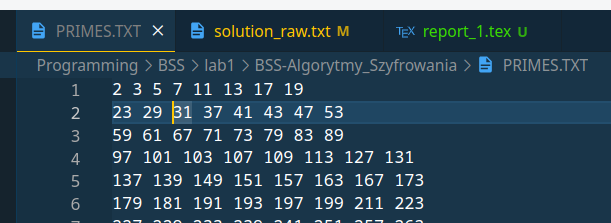
\includegraphics[width=1\textwidth]{one.png}
\paragraph{n = p * q = 31 * 37 = 1147}
\paragraph{$\rho(n) = (p-1) * (q-1) = 30 * 36 = 1080$}
\paragraph{Wybrałem liczbę e = 29}
Sprawdziłem, że jest względnie pierwsza względem 1080 \\ 
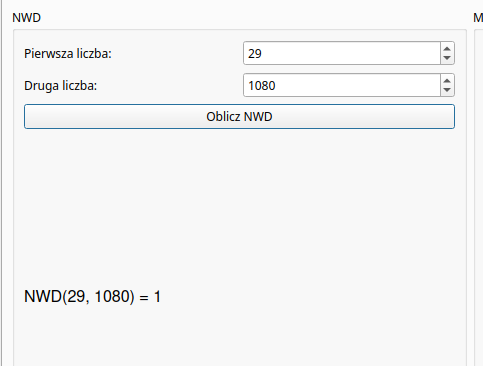
\includegraphics[width=1\textwidth]{two.png}
\paragraph{Liczba d = 149 \\}  
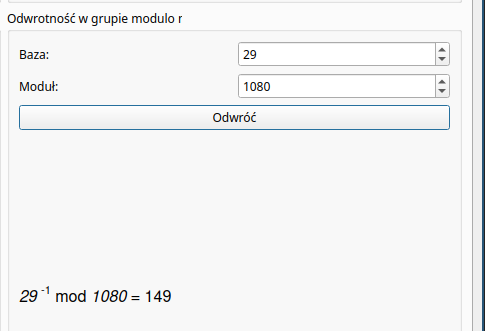
\includegraphics[width=1\textwidth]{three.png}
\paragraph{Klucz publiczny:  e = 29, n = 1147 \\ Klucz prywatny: d = 149, n = 1147}

\section{Szyfrowanie}
\paragraph{Fraza: DYZIO, litera: C}
\paragraph{Zakodowana Fraza: 68, 89, 90, 73, 79 \\ Zakodowana litera: 67}
\paragraph{Przygotowana wiadomość: PTAKI LATAJA KLUCZEM}
\paragraph{Wiadomość zaszyfrowana kluczem sesyjnym: KPWEB FWPWCW EFQDVZG \\}
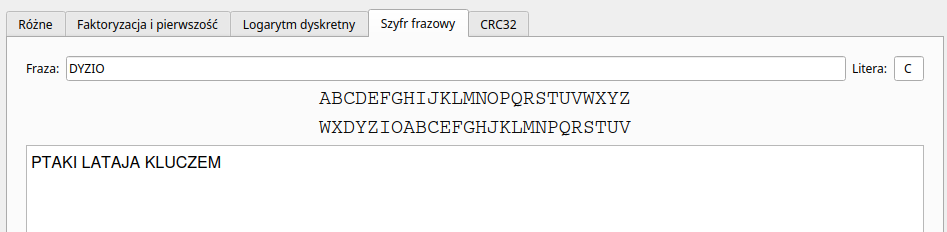
\includegraphics[width=1\textwidth]{four.png}
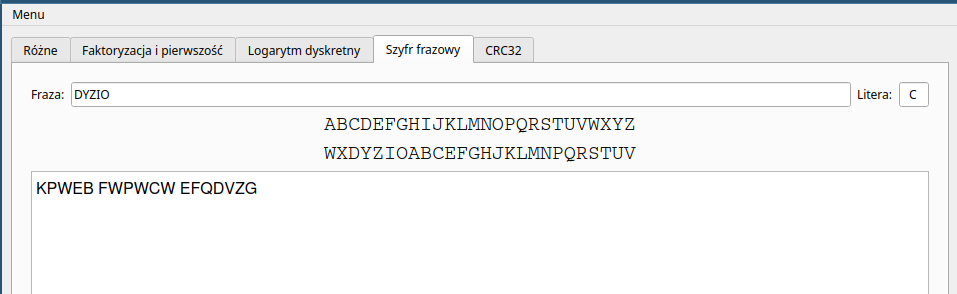
\includegraphics[width=1\textwidth]{five.png}
\paragraph{Klucz pobrany od kolegi:  $e_2 = 11, n_2 = 1763$}
\paragraph{Zaszyfrowany klucz sesyjny \\ Fraza: 168, 1621, 1632, 665, 178 \\ Litera: 1734 \\}
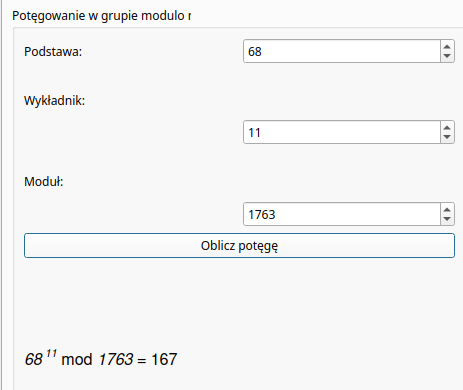
\includegraphics[width=1\textwidth]{six.png}
\paragraph{Klucz sesyjny przed zakodowaniem: DYZIO, C \\ Po Zakodowaniu: 68, 89, 90, 73, 79, \_67\_ \\ Po Zaszyfrowaniu: 168, 1621, 1632, 665, 178, \_1734\_}
\paragraph{Wiadomość przed zaszyfrowaniem: PTAKI LATAJA KLUCZEM \\ Wiadomość po zaszyfrowaniu: KPWEB FWPWCW EFQDVZG}

\section{Odszyfrowanie}
\paragraph{Otrzymałem klucz sesyjny:  423 65 693 1100 8 \_1073\_}
\paragraph{Odszyfrowałem go korzystając z mojego klucza prywatnego Klucz prywatny: d = 149, n = 1147}
\paragraph{Odszyfrowany klucz sesyjny: 107, 114, 48, 122, 97, \_111\_ \\}
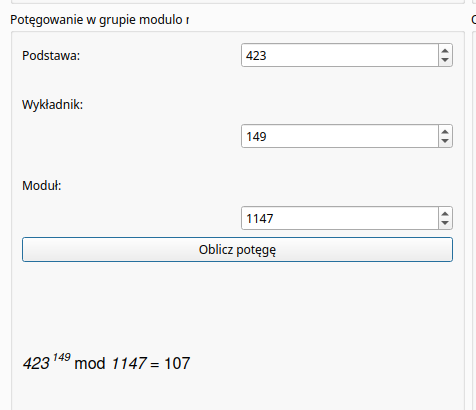
\includegraphics[width=1\textwidth]{seven.png}
\paragraph{Odszyfrowany klucz sesyjny odkodowałem: kryza, o}
\paragraph{Otrzymałem wiadomość: QNVVK XSLN BK WNNB GKC \\ } 
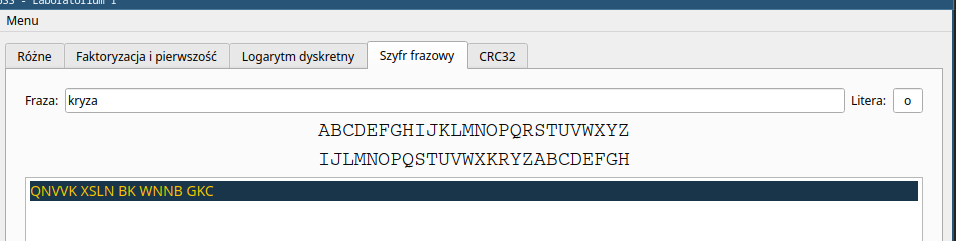
\includegraphics[width=1\textwidth]{eight.png} 
\paragraph{Odszyfrowałem ją: HELLO NICE TO MEET YOU \\}
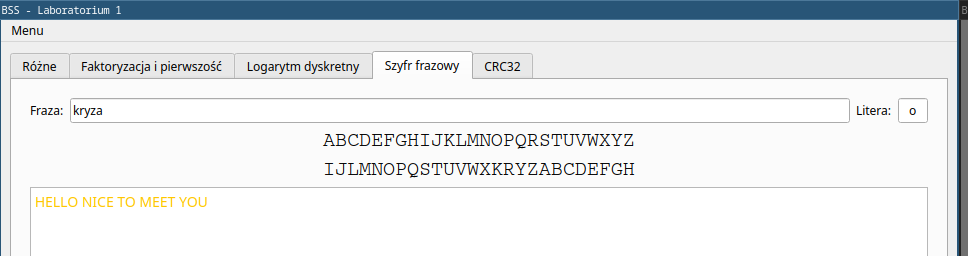
\includegraphics[width=1\textwidth]{nine.png}
\paragraph{Otrzymany klucz sesyjny zaszyfrowany: 423 65 693 1100 8 \_1073\_ \\ po odszyfrowaniu: 107, 114, 48, 122, 97, \_111\_ \\ po odkodowaniu: kryza, o }
\paragraph{Wiadomość zaszyfrowana: QNVVK XSLN BK WNNB GKC \\ Wiadomość odszyfrowana: HELLO NICE TO MEET YOU}
\section{Łamanie klucza prywatnego}
\end{document}